% !TeX spellcheck = de_DE
\documentclass[10pt, a4paper, reqno]{amsart}
\usepackage[utf8x]{inputenc}
\usepackage{polyglossia}
\setdefaultlanguage{ngerman}
\usepackage{enumitem}

\usepackage{xcolor}

\usepackage{caption}
\captionsetup[figure]{name=Abbildung}
\usepackage{tikz, tkz-euclide}
\usetikzlibrary{calc}

\usepackage{amsmath, amsfonts, amssymb}
\usepackage{amsthm, thmtools}
\declaretheorem[name=Aufgabe, thmbox = L]{aufgabe}
\declaretheorem[name=Lemma]{lemma}
\counterwithin*{lemma}{aufgabe}
\counterwithin*{equation}{aufgabe}
\newcommand{\aufgabelabelname}{\theaufgabe . Aufgabe}
\renewcommand\qedsymbol{$\blacksquare$}
\renewcommand\proofname{Beweis}

\usepackage{physics}
\usepackage{fancyhdr}
\fancyheadoffset{0cm} 
\usepackage[
  a4paper,
  right=6cm,
  footskip=3em,
  twoside=false,
  lmargin=1.4cm,
  %bottom=4cm,
  %top=4cm
  xetex
]{geometry}
\usepackage{unicode-math}
\listfiles
\makeatletter
\renewenvironment{proof}[1][\proofname]{\par
\pushQED{\qed}%
\normalfont \topsep6\p@\@plus6\p@\relax
\trivlist
\item\relax
{\bfseries#1}\hspace\labelsep\ignorespaces
}{%
\popQED\endtrivlist\@endpefalse
}
\newenvironment{proof_thm}[1]{
\begin{proof}[\proofname~(#1)]}{\end{proof}}
\makeatother
	
\fancypagestyle{Hilfsmittel}{%
  \rhead{
    \fontsize{9}{7}Valentin Herrmann
  }
}

\fancypagestyle{normal}{
  \chead{
    \fontsize{9}{7}\large\aufgabelabelname
  }
  \rhead{
    \fontsize{9}{7}Valentin Herrmann}
}

%  \begin{tikzpicture}
%      \def\range{41}%
%      \def\radius{0.6cm}%
%      \def\a{\fpeval{360/\range}}%
%      \foreach \i in {0,1,...,\range}{%
%        \definecolor{colora}{hsb}{\fpeval{\i/\range},1,0.7}%
%        \draw[colora, very thin] (\i*\a-90:\radius) -- (2*\i*\a-90:\radius);%
%      }%
%      \draw[very thin] (0,0) circle[radius=\radius];%
%    \end{tikzpicture}

%hyperref must be the last package in the preamble
\usepackage{hyperref}
\hypersetup{
	bookmarks=true,
	unicode=true,
	pdfborder={0 0 0},
	pdfstartview={FitH},
	pagebackref=true,
	colorlinks=true,
	urlcolor=blue,
	linkcolor=black,
	linktoc=all
}
\renewcommand{\figureautorefname}{Abbildung}

\begin{document}
\thispagestyle{Hilfsmittel}
\vspace*{3pt}
\begin{center}
  \large\textbf{Hilfsmittel:}
\end{center}
\vspace*{3pt}
\begin{itemize}
\item Gaußsche Summenformel: \url{https://de.wikipedia.org/wiki/Gau%C3%9Fsche_Summenformel}, zuletzt
  aufgerufen am Fr, 28 August 2020
\item Kongruenz: \url{https://de.wikipedia.org/wiki/Kongruenz_(Zahlentheorie)}, zuletzt
  aufgerufen am Fr, 28 August 2020
\item Vollständige Induktion:
  \url{https://de.wikipedia.org/wiki/Vollst%C3%A4ndige_Induktion}, zuletzt
  aufgerufen am So, 30 August 2020
\end{itemize}
\newpage
\pagestyle{normal}
\begin{aufgabe}
  Leo und Smilla finden 2020 Goldnuggets mit den Massen 1, 2,\ldots, 2020 Gramm,
  die sie nach folgender Regel auf eine rote und eine blaue Schatztruhe
  verteilen:
 
  Zuerst wählt Leo eine der Schatztruhen und nennt Smilla die Farbe der Truhe.
  Anschließend wählt Smilla eines der noch nicht verteilten Nuggets und legt es
  in diese Truhe. Dies wiederholen sie, bis alle Nuggets verteilt sind. Danach
  wählt Smilla eine der beiden Schatztruhen und bekommt alle Nuggets in dieser
  Truhe.

  Wie viel Gramm Gold kann Smilla auf diese Weise mindestens für sich
  garantieren?
\end{aufgabe}
\begin{lemma}\label{sec1:Zahlensumme}
  Für alle $n∈ℕ^*$ gilt:
  \[ \sum^{n}_{k=1}k=\frac{n(n+1)}{2}\]
\end{lemma}
\begin{lemma}
  \label{sec1:zahlengruppen}
  Jeder Abschnitt der natürlichen Zahlen, welcher mit $1$ beginnt und mit einer
  Zahl $n=4k+3$, $k∈ℕ_0$ aufhört, kann in zwei gleich große Gruppen geteilt
  werden.
\end{lemma}
\begin{proof}
  Für einen einfacher lesbaren Beweis werden die Nuggets jeweils nach ihrer
  Masse benannt. Nugget $1234$ steht also für das Nugget mit der Masse $1234$g.
  Zusätzlich werden einige Variablen nach dem entsprechenden Vergabevorgang benannt.
  Zum Beispiel steht $r_{2019}$ für das Gewicht der roten Truhe nach der Vergabe
  des 2019ten Nuggets, welches ein Gewicht von $n_{2019}$ hat.
  
  Zuerst wird die Obergrenze für den Schatz, welchen Smilla noch garantieren
  kann, bestimmt. Dazu wird die Situation vor der Vergabe des letzten Nuggets
  $n_{2020}$ betrachtet. Zu diesem Zeitpunkt liegen natürlich alle Nuggets bis
  auf das letzte in den beiden Truhen. Als Gleichung unter Anwendung
  von ~\autoref{sec1:Zahlensumme} ausgedrückt:
  \begin{equation}\label{sec1:equation1}
    r_{2019}+b_{2019}=\sum_{k=1}^{2020}\left(k\right)-n_{2020}=\frac{2020\cdot2021}{2}-n_{2020}
  \end{equation}
  Da Smilla sich nach der Vergabe des letzten Nuggets ihre Truhe aussuchen darf
  wird Leo die leichtere Truhe bekommen. Also wird Leo versuchen die Truhen so
  gleichmäßig wie möglich zu füllen. Daher wird Leo bei der Vergabe des letzten
  Nuggets logischerweise die leichtere Truhe für das letzte Nugget wählen.

  Angenommen $r_{2019}\leq b_{2019}$ gilt vor der Vergabe des letzten Nuggets (Die Truhen sind
  austauschbar), dann wird Leo die rote, leichtere Truhe wählen und Smilla wird das letzte
  Nugget $n_{2020}$ in diese Truhe legen. Daraus folgt bei Einsetzen von~\eqref{sec1:equation1}:
  \begin{equation}\label{sec1:equation2}
    \begin{split}
      r_{2020}&=r_{2019}+n_{2020}=(1010\cdot2021-b_{2019}-n_{2020})+n_{2020}\\
       &= 1010\cdot2021-b_{2019}
    \end{split}
  \end{equation}
  Also hat $r_{2020}$ den maximalen Wert, wenn $b_{2019}$ minimal ist. Da
  $b_{2019}$ trotzdem noch größer gleich $r_{2019}$ sein muss, ist der minimale Wert von
  $b_{2019}$ gleich $r_{2019}$. Für den Idealfall $r_{2019}=b_{2019}$ folgt
  daher aus~\eqref{sec1:equation1}:
  \begin{equation}\label{sec1:equation3}
    \begin{split}
      b_{2019} + r_{2019}= 2b_{2019} &=1010\cdot2021-n_{2020}\\
      \Rightarrow b_{2019} &=505\cdot2021-\frac{n_{2020}}{2}
    \end{split}
  \end{equation}
  Wird~\eqref{sec1:equation3} in \eqref{sec1:equation2} eingesetzt:
  \begin{equation*}
    r_{2020}= 1010\cdot2021 -(505\cdot2021 - \frac{n_{2020}}{2})=505\cdot2021+\frac{n_{2020}}{2}
  \end{equation*}
  Im Idealfall für Smilla ist $n_{2020}$ maximal groß und hat daher den Wert
  2020. Damit gilt für die Obergrenze $r_{2020}$:
  \begin{equation*}
    r_{2020}=505\cdot2021+1010 = 505\cdot2023 = 1021615
  \end{equation*}
  Die folgende Strategie zeigt, dass Smilla die Obergrenze erreichen kann.

  Smilla teilt alle Nuggets bis auf $2020$ in zwei gleich schwere Gruppen. Das
  ist möglich, da alle Nuggets von $1$ bis $2019$ dabei sind und das größte
  Nugget $2019$ gleich $4\cdot504+3$ ist, weshalb~\autoref{sec1:zahlengruppen}
  anwendbar ist. Jede Gruppe entspricht dabei einer Truhe und hat einen Wert von
  $\frac{\sum^{2019}_{k=1}k}{2} = \frac{\frac{2019\cdot2020}{2}}{2} =
  505\cdot2019$. Werden die Nuggets nun verteilt, so legt Smilla in die von Leo
  ausgewählte Truhe ein Nugget der entsprechenden Gruppe. Wählt Leo irgendwann eine Truhe aus, in
  welcher schon alle Nuggets der entsprechenden Gruppe liegen, so legt Smilla das
  Nugget $2020$ in diese Truhe. Danach hat diese Truhe einen Wert von
  $505\cdot2019 + 2020 = 505\cdot2023 = 1021615$. Leo muss eine solche Truhe spätestens auswählen,
  wenn alle Nuggets bis auf $2020$ aufgeteilt sind, weshalb beide Truhen mit
  ihrer Gruppen gefüllt sind. Also erreicht eine der Truhen immer einen Wert von
  $1021615$, womit die Obergrenze erreicht ist.
\end{proof}
\begin{proof_thm}{\autoref{sec1:Zahlensumme}}
  \begin{align*}
    \sum^{n}_{k=1}k&=\frac{1}{2}\cdot\left(\sum^{n}_{k=1}k + \sum^{n}_{k=1}k\right) = \frac{1}{2}\cdot\left(\sum^{n}_{k=1}k+\sum^{n}_{k=1}(n+1-k)\right)\\
                   &= \frac{1}{2}\cdot\sum^{n}_{k=1}(k+(n+1-k)) = \frac{1}{2}\cdot\sum^{n}_{k=1}(n+1)\\
                   &= \frac{n(n+1)}{2}
  \end{align*}
\end{proof_thm}
\begin{proof_thm}{\autoref{sec1:zahlengruppen}}
  Die Zahlenreihe wird um Null erweitert, sodass die Reihe aus insgesamt
  $n+1=4(k+1)$ Zahlen besteht. Nun wird die Zahlenfolge in der Mitte „gefaltet“.
  Die kleinste Zahl wird mit der Größten gepaart $\Rightarrow (0;n)$, die zweit
  Kleinste mit der zweit Größten $\Rightarrow (1;n-1)$, $(2;n-2)$, etc.. So
  entstehen $\frac{4(k+1)}{2}=2(k+1)$ Paare, jeweils mit einer Summe von
  $(j)+(n-j) = n$ mit $0\leq j \leq n$, $j∈ℕ_0$. Da die Paare alle gleich groß
  sind und es eine gerade Anzahl von ihnen gibt, können sie in zwei Gruppen mit
  gleich vielen Paaren und daher gleicher Summe unterteilt werden. Dabei kann
  nun die Null wieder entfernt werden, schließlich verändert sie die Summe
  ihrer Gruppe nicht.
\end{proof_thm}

\newpage
\begin{aufgabe}
  Beweise: Es gibt keine rationalen Zahlen $x$, $y$, $z$ mit $x + y + z = 0$ und
  $x + y + z = 100$.
\end{aufgabe}
\begin{lemma}\label{sec2:rational1}
  Jeder Quotient $\frac{a}{b}$ zweier rationaler Zahlen $a,b∈ℚ\backslash\{0\}$
  ist rational definiert.
\end{lemma}
\begin{lemma}\label{sec2:rational2}
  Jedes Produkt $ a\cdot b $ einer rationalen Zahl $a$ ungleich Null und einer
  irrationalen Zahl $b$ ist irrational definiert.
\end{lemma}
\begin{proof}
  Zuerst wird $x+y+z = 0 \Rightarrow z = -(x+y)$ in $x^2+y^2+z^2 = 100$
  eingesetzt:
  \begin{equation}
    \label{eq:1}
    \begin{split}
      x^2+y^2+(-(x+y))^2 = x^2+y^2+(x^2+2xy+y^2) &= 100\\
      \Rightarrow x^2+xy+y^2&=50
    \end{split}
  \end{equation}
  Nun wird angenommen, dass $x$ und $y$ rational sind und aus (1) ein Widerspruch hergeleitet:

  Aus~\eqref{eq:1} folgt direkt, dass $x$ oder $y$ nicht gleich Null sein können. Ist eine der Variablen
  Null so gilt: $0^2+0\cdot a+a^2=a^2=50\Rightarrow a = \pm5\sqrt{2}$. $a$ ist
  dabei ein Platzhalter für $x$ oder $y$. Da $\sqrt{2}$ irrational ist, muss
  wegen~\autoref{sec2:rational1} $a$ irrational sein, womit ein Widerspruch
  entsteht.
  
  Durch Teilen von~\eqref{eq:1} durch $x^2$ entsteht
  $(\frac{y}{x})^2+\frac{y}{x}+1=\frac{50}{x^2}$. Das Teilen durch $x^2$ ist
  erlaubt, da $x$ nicht Null sein kann, wenn $y$ rational ist.
  
  Aus~\autoref{sec2:rational1} folgt, dass $q=\frac{y}{x}$ als eine gekürzte
  rationale Zahl $\frac{m_q}{n_q}$ mit $m_q,n_q\in\mathbb{Z}\backslash\{0\}$,
  beschreibbar sein muss. Auch $x$ wird in der Gleichung zu dem gekürzten Bruch $\frac{m_x}{n_x}$, mit
  $m_x,n_x\in\mathbb{Z}\backslash\{0\}$ umgeschrieben:
  \begin{equation}
    \label{eq:2}
    \begin{split}
      \left(\frac{m_q}{n_q}\right)^2+\frac{m_q}{n_q}+1&=\frac{50}{\left(\frac{m_x}{n_x}\right)^2}=\frac{2\cdot 5^2n_x^2}{m_x^2}\\
      \Rightarrow \frac{m_q^2+m_q\cdot n_q +
        n_q^2}{2}&=\frac{5^2n_x^2n_q^2}{m_x^2}
    \end{split}
  \end{equation}
  Da jeder Primfaktor von $n_x$, $n_q$ und $m_x$ durch das Quadrat verdoppelt
  wird, müssen in der Primfaktorzerlegung von $(\frac{5n_xn_q}{m_x})^2$ alle
  Primfaktoren gerade Exponenten haben. Gleiches muss für
  $\frac{m_q^2+m_q\cdot{}n_q+n_q^2}{2}$, insbesondere für den Primfaktor $2$
  gelten. Doch solange der Zähler des Bruches nicht durch zwei teilbar ist, hat
  $2$ im Bruch den ungeraden Exponenten $-1$. Um herauszufinden, ob der Zähler
  überhaupt durch zwei teilbar sein kann wird unter Anwendung von
  Kongruenz (siehe:
  \url{https://de.wikipedia.org/wiki/Kongruenz_(Zahlentheorie)}, zuletzt
  aufgerufen am Fr, 28 August 2020) zwischen drei Fällen unterschieden:
  \begin{itemize}[itemsep=2ex]
  \item $m_q$ und $n_q$ sind beide ungerade:
    \[m_q^2+m_qn_q+n_q^2\equiv1^2+1\cdot1+1^2\equiv1\pmod{2}\] In
    diesem Fall ist der Zähler ungerade.
  \item $m_q$ ist gerade und $n_q$ ungerade:
    \[m_q^2+m_qn_q+n_q^2\equiv0^2+0\cdot1+1^2\equiv1\pmod{2}\] Auch in diesem Fall ist der Zähler ungerade.
  \item $m_q$ ist ungerade und $n_q$ gerade:
    Da der Zähler symmetrisch in Rücksicht auf $m_q$ und $n_q$ ist, gilt gleiches wie im vorherigen
    Fall.
  \item $m_q$ und $n_q$ sind beide gerade:
    Es dürfen nicht beide Variablen gerade sein, da sie nach ihrer Definition die
    Zahl $q=\frac{y}{x}$ gekürzt darstellen sollen. Sie müssen daher teilerfremd sein.
  \end{itemize}
  In jedem möglichen dieser Fälle ist der Exponent von $2$ auf der linken Seite
  von~\eqref{eq:2} also im Gegensatz zu der Rechten ungerade. Daher kann $\frac{y}{x}$ also keine rationale
  Zahl sein, wenn auch $x$ eine rationale
  Zahl ist. Doch gleichzeitig muss $\frac{y}{x}$ eine rationale Zahl sein, wenn $x$ und $y$ beide rational
  sind.
  Daher können $x$ und $y$ nicht beide rational sein.
\end{proof}
\begin{proof_thm}{\autoref{sec2:rational1}}
  Wird $a$ durch $\frac{m_a}{n_a}$ und $b$ durch $\frac{m_b}{n_b}$ beschrieben,
  wobei $m_a,n_a,m_b,n_b∈ℤ\backslash\{0\}$ gilt, so kann der Quotient umgeschrieben werden:
  \begin{equation*}
    \frac{a}{b} = \dfrac{\frac{m_a}{n_a}}{\frac{m_b}{n_b}}=\frac{m_a\cdot n_b}{m_b\cdot n_a}
  \end{equation*}
  Da $m_a\cdot n_b$ und $m_b\cdot n_a$ ganze Zahlen ungleich
  Null sind, ist der Quotient rational.
\end{proof_thm}
\begin{proof_thm}{\autoref{sec2:rational2}}
  Beweis durch Widerspruch: Angenommen das Produkt $c$ ist eine rationale Zahl:
  \begin{equation*}
    ab=c \Rightarrow b =\frac{c}{a}
  \end{equation*}
  Der Bruch $\frac{c}{a}$ muss nach~\autoref{sec2:rational1} rational sein, also
  gibt es einen Widerspruch, denn $b$ ist irrational. Daher darf $c$ nicht
  rational sein.
\end{proof_thm}

\newpage
\begin{aufgabe}
  Zwei Geraden $m$ und $n$ schneiden sich in genau einem Punkt $P$. Ein Punkt
  $M$ bewegt sich auf m mit konstanter Geschwindigkeit, ein weiterer Punkt $N$
  bewegt sich auf $n$ mit derselben Geschwindigkeit; dabei passieren sie beide
  den Punkt $P$, aber nicht gleichzeitig.
 
  Beweise: Es gibt einen festen, von $P$ verschiedenen Punkt $Q$ so, dass die
  Punkte
  $P$, $Q$, $M$ und $N$ zu jedem Zeitpunkt auf einem gemeinsamen Kreis liegen.\\
\end{aufgabe}
\begin{lemma}\label{sec3:lemma1}
  Für jeden festen Punkt $P$ und jeden von $P$ verschiedenen Punkt $Q$ existiert ein Gerade $g$, sodass
  der Mittelpunkt von jedem Kreis, welcher durch beide Punkte führt, auf der
  Geraden liegt.
\end{lemma}
\begin{lemma}\label{sec3:lemma3}
  Für jeden Punkt $P$ und jede Gerade $g$ existiert ein von $P$ verschiedenen Punkt $P'$, sodass jeder
  Kreis, dessen Mittelpunkt auf der Geraden liegt und auf welchem $P$ liegt,
  auch durch $P'$ führt, solange $P$ nicht auf $g$ liegt.
\end{lemma}
\begin{lemma}\label{sec3:lemma2}
  Sind in einem Dreieck zwei Höhen gleich, so muss das Dreieck gleichschenklig
  sein. Dabei sind die Seiten auf welchen die beiden Höhen stehen die Schenkel des
  gleichschenkligen Dreiecks.
\end{lemma}
\begin{proof}
  Nur wenn der Mittelpunkt $U$ des Kreises durch $P$, $M$ und $N$, zu jedem Zeitpunkt auf der gleichen Geraden
  liegt und $P$ nicht auf dieser Geraden liegt, existiert nach~\autoref{sec3:lemma1} ein weiterer fester Punkt $Q$,
  welcher genauso wie $P$ auf dem Kreis liegt.

  Um die Existenz der Geraden zu beweisen wird nun die Gerade $(U_tU_0)$ in
  Abhängigkeit der Zeit $t$ konstruiert. Dabei ist $U_0$ der Kreismittelpunkt
  von $t=0$. Ist die Gerade unabhängig von $t$, dann liegen also alle $U$ auf
  der gleichen Gerade.

  \begin{figure}[h]
    \centering
    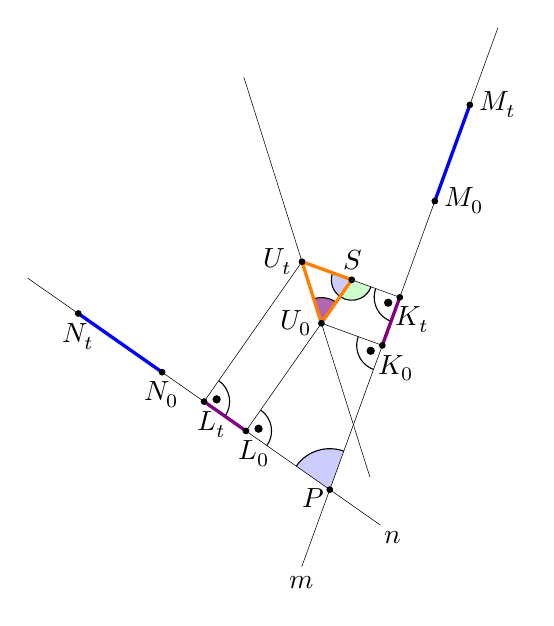
\begin{tikzpicture}[rotate=70,scale=1.3]
      % \tkzSetUpLine[add=.5 and .5]%
      \tkzSetUpPoint[fill=black]%
    
      \def\vara{75} \def\varx{1}%
    
      \tkzDefPoint(0,0){P} \tkzDefPoint(0:4){M_t} \tkzDefPoint(\vara:3){N_t}%
      \tkzDefShiftPoint[M_t](0:-\varx){M_0}%
      \tkzDefShiftPoint[N_t](\vara:-\varx){N_0}%

      \foreach \i in {0, t} { \foreach \kl/\mn in {K/M, L/N} {%
          \tkzDefLine[mediator](P,\mn_\i) \tkzGetPoints{\kl_\i_1}{\kl_\i_2}%
          \tkzInterLL(\kl_\i_1,\kl_\i_2)(P,\mn_\i) \tkzGetPoint{\kl_\i} }%
        \tkzInterLL(K_\i_1,K_\i_2)(L_\i_1,L_\i_2) \tkzGetPoint{U_\i} }%

      \tkzInterLL(L_0_1,L_0_2)(K_t_1,K_t_2) \tkzGetPoint{S}%
      % \tkzInterLL(K_0_1,K_0_2)(L_t_1,L_t_2) \tkzGetPoint{R}%

      \tkzFillAngles[fill=blue!20,size=0.4](M_t,P,N_t)%
      \tkzFillAngles[fill=green!20,size=0.2](U_0,S,K_t)%
      \tkzFillAngles[fill=blue!20,size=0.2](U_t,S,U_0)%
      \tkzFillAngles[fill=blue!50!red!60,size=0.25](S,U_0,U_t)%
      
      \tkzMarkAngle[size=0.4](M_t,P,N_t)%
      \tkzMarkAngle[size=0.2](U_0,S,K_t)%
      \tkzMarkAngle[size=0.2](U_t,S,U_0)%
      \tkzMarkAngle[size=0.25](S,U_0,U_t)%

      \tkzMarkRightAngles[german](P,L_t,U_t P,L_0,U_0 U_t,K_t,P U_0,K_0,P)%

      % \tkzDefLine[parallel=through L_t](L_0,S) \tkzGetPoint{L_t'}%
      % \tkzDefLine[parallel=through K_t](K_0,R) \tkzGetPoint{K_t'}%
      \tkzDrawLines(P,M_t P,N_t)%
      \tkzDrawLines[add= 0 and 0](K_t,U_t L_t,U_t K_0,U_0 L_0,S)%
      \tkzDrawLines[add=2.5 and 3](U_0,U_t)%
      \tkzDrawPolygon[orange, very thick](U_t,U_0,S)%
      \tkzDrawSegments[blue, very thick](N_t,N_0 M_t,M_0)%
      \tkzDrawSegments[blue!50!red, very thick](L_0,L_t K_0,K_t)%
        
      \tkzDrawPoints(P, M_t, N_t, M_0, N_0, K_0, K_t, L_0, L_t, U_0, U_t, S)%
        
      \tkzLabelPoints[left, yshift=-3pt](P) \tkzLabelPoints[right](M_t, M_0)%
      \tkzLabelPoints[below right, xshift=-0.5em](K_0, K_t)%
      \tkzLabelPoints[below](N_t, N_0) \tkzLabelPoints[below, xshift=3pt](L_0,
      L_t)%
      \tkzLabelPoints[left](U_0) \tkzLabelPoints[above](S)%
      \tkzLabelPoints[left](U_t) \tkzLabelLine[below, pos=1.2](M_t, P){$m$}%
      \tkzLabelLine[below right, pos=1.18](N_t, P){$n$}%
    \end{tikzpicture}
    \caption{}
    \label{fig:1}
  \end{figure}

  Da der Kreis um $U$ durch $P$, $M$ und $N$ gehen muss, entspricht er also dem
  Umkreis des Dreiecks $PMN$. Der Umkreismittelpunkt $U$ ist der Schnittpunkt der Mittelsenkrechten
  der Dreiecksseiten. Also werden die Schnittpunkte der Mittelsenkrechten auf $[NP]$
  und $[MP]$ für die beiden Zeitpunkte konstruiert, denn zwei Mittelsenkrechten
  reichen aus, um den Umkreismittelpunkt zu bestimmen.
  
  In~\autoref{fig:1} stehen $L_t$, $L_0$, $K_t$ und $K_0$ jeweils für den
  Mittelpunkt der Strecke von $N_t$, $N_0$, $M_t$ und $M_0$ bis $P$. Der Punkt
  $S$ ist der Schnittpunkt der Senkrechten auf $L_0$ und der Senkrechten auf
  $K_t$.

  $(U_tU_0)$ ist die Rotation von $(L_0U_0)$ an $U_0$ um den Winkel $\angle
  SU_0U_t$. Da weder $L_0$ noch $U_0$ von der Zeit abhängig sind, ist die
  Gerade $(U_tU_0)$ auch unabhängig, wenn gleiches für den Winkel $\angle
  SU_0U_t$ gilt. Daher wird dieser Winkel nun bestimmt.
  
  Da das organgene Dreieck $U_0SU_t$ von den beiden Paaren an Parallelen
  $(U_0K_0) || (U_tK_t)$ und $(L_0S) || (L_tU_t)$ eingerahmt wird, entsprechen
  die violetten Strecken $[K_tK_0]$ und $[L_tL_0]$ (siehe~\autoref{fig:1}) den Höhen des orangen
  Dreiecks auf den Seiten $U_tS$ und $U_0S$. Für die Strecken $[L_tL_0]$,
  $[K_tK_0]$ gilt:
  \begin{align*}
    \overline{L_tL_0}&=\overline{L_tP}-\overline{L_0P}=\frac{\overline{N_tP}}{2} - \frac{\overline{N_0P}}{2} = \frac{\overline{N_tN_0}}{2}\\
    \overline{K_tK_0}&=\overline{K_tP}-\overline{K_0P}=\frac{\overline{M_tP}}{2} - \frac{\overline{M_0P}}{2} = \frac{\overline{M_tM_0}}{2}
  \end{align*}
  Die blauen Abschnitte $[N_tN_0]$ und $[M_tM_0]$ sind die Strecken, welche $N$ und $M$ zwischen den
  beiden Zeitpunkten zurücklegen. Da $M$ und $N$ sich gleich
  schnell fortbewegen, sind die beiden Strecken gleich lang. Gleiches gilt für
  die violetten Strecken, weil sie jeweils halb so lang wie die Blauen sind.
  Aus~\autoref{sec3:lemma2} folgt daher, dass das orangene Dreieck $U_0SU_t$
  gleichschenklig ist.

  Nun wird der Wert des Winkels $\angle SU_0U_t$ bestimmt. Aus der
  Gleichschenkligkeit von $U_0SU_t$ folgt:
  \begin{equation}
    \label{eq:7}
    \begin{split}
      \angle SU_0U_t& +\angle U_0U_tS + \angle U_tSU_0 = 180°\\
      2\angle SU_0U_t&= 180° - \angle U_tSU_0\\
      \angle SU_0U_t&= 90° - \frac{\angle U_tSU_0}{2}
    \end{split}
  \end{equation}
  Da der blaue Winkel $\angle U_tSU_0$ und der grüne Winkel $\angle L_0SK_t$
  Nebenwinkel bei $S$ sind, gilt:
  \begin{equation}
    \label{eq:5}
    \angle U_tSU_0 + \angle L_0SK_t = 180° \Rightarrow \angle U_tSU_0 = 180° - \angle L_0SK_t
  \end{equation}
  Und letztendlich hat die Winkelsumme im Viereck immer einen Wert von $360°$.
  Daher gilt für das Viereck $PK_tSL_0$:
  \begin{equation}
    \label{eq:6}
    \begin{split}
      &\angle L_0SK_t + \angle K_tPL_0 + 2\cdot 90° = 360°\\
      \Rightarrow &\angle L_0SK_t= 180° - \angle K_tPL_0
    \end{split}
  \end{equation}
  Nun werden~\eqref{eq:6} und~\eqref{eq:5} in~\eqref{eq:7} eingesetzt:
\begin{align*}
    \angle SU_0U_t &= 90° -\frac{\angle U_tSU_0}{2}\\
    \Rightarrow \angle SU_0U_t &= 90° -\frac{180°-\angle L_0SK_t}{2}\\
    \Rightarrow \angle SU_0U_t &= 90° -\frac{180°-(180° - \angle K_tPL_0)}{2}\\
    \Rightarrow \angle SU_0U_t &= 90° -\frac{\angle K_tPL_0}{2}\\
  \end{align*}
  Da die beiden Geraden $m$ und $n$ nicht von der Zeit abhängig sind, ist es
  also auch nicht der Winkel $\angle K_tPL_0$ und damit auch $\angle SU_0U_t$ nicht.
  Damit ist die Gerade $(U_tU_0)$ unabhängig von der Zeit definiert, also ist
  sie für alle $t$ identisch, womit alle $U$ auf der gleichen Geraden liegen.
  %Also ist die Gerade $(U_tU_0)$ eine Rotation der Gerade $(L_0U_0)$ an $U_0$ um
  %den Winkel $90° -\frac{\angle K_tPL_0}{2}$ gegen den Uhrzeigersinn. Da weder $U_0$, die Senkrechte durch $L_0$, noch der Winkel $\angle K_tPL_0$
  %von $t$ abhängig sind, ist die Gerade $(U_tU_0)$ also auch unabhängig von $t$.
  %Daraus folgt, dass alle $U$ auf der gleichen Geraden liegen.
  Also muss wegen~\autoref{sec3:lemma3} ein weiterer fester Punkt
  $Q$ existieren, sodass alle Kreise, welche durch $P$ führen und dessen
  Mittelpunkte auf $(U_tU_0)$ liegen, auch durch $Q$ führen, solange
  $P$ nicht auf der Geraden $(U_tU_0)$ liegt.

  Doch $P$ kann nicht auf $(U_tU_0)$ liegen, denn dann gäbe es
  einen Zeitpunkt in welchem der Umkreismittelpunkt deckungsgleich mit $P$ wäre.
  Da $P$ allerdings gleichzeitig immer noch auf dem Kreis läge, müsste der
  Radius des Kreises einen Wert von Null haben, womit auch $M$ und $N$
  gleichzeitig auf $P$ liegen, was durch die Aufgabenstellung verboten ist.
\end{proof}
\begin{proof_thm}{\autoref{sec3:lemma1}}
  Der Punkt $U$ wird mit $P$ und $Q$ verbunden und das Lot durch $U$ auf $[PQ]$
  wird in~\autoref{fig:3} eingezeichnet:
  \begin{figure}[h]
    \centering
    \begin{tikzpicture}
      \tkzDefPoints{0/0/P, 4/0/Q}%
      \tkzDefMidPoint(P,Q) \tkzGetPoint{M}%
      \tkzDefLine[mediator](P,Q) \tkzGetPoints{ms1}{ms2}%
      \tkzDefBarycentricPoint(ms1=8,ms2=1) \tkzGetPoint{U}%

      \tkzMarkRightAngle[german, size=0.4](U,M,P)%
      \tkzDrawLines[add=0 and -0.35](ms1,ms2)%
      \tkzDrawSegments(P,Q P,U Q,U)%
      %\tkzMarkSegments[color=blue, mark=|](P,M M,Q)%
      %\tkzMarkSegments[color=blue, mark=|](P,M M,Q)%
      \tkzDrawArc[delta=20, black](U,P)(Q)
      \tkzDrawPoints(P, Q, U, M)%

      \tkzLabelLine[pos=1.37, below](U,M){$g$}%
      \tkzLabelPoints[above right](U,M)%
      \tkzAutoLabelPoints[center=U, pos=0.95](P, Q)%
    \end{tikzpicture}
    \caption{}
    \label{fig:3}
  \end{figure}
  Über den Satz des Pythagoras können in den Dreiecken $PMU$ und $MQU$ die Längen von $[PU]$ und $[UQ]$
  umgeschrieben werden:
  \begin{align*}
    \overline{PU}^2&=\overline{PM}^2+\overline{UM}^2 &\Rightarrow \overline{PU}=\sqrt{\overline{PM}^2+\overline{UM}^2}\\
    \overline{QU}^2&=\overline{QM}^2+\overline{UM}^2 &\Rightarrow \overline{QU}=\sqrt{\overline{QM}^2+\overline{UM}^2}
  \end{align*}
  Liegen $P$ und $Q$ auf dem selben Kreis um $U$, so müssen $\overline{PU}$ und
  $\overline{QU}$ gleichlang sein (Da mit positiven Längen gerechnet wird,
  müssen keine Beträge genommen werden.):
  \begin{align*}
    \sqrt{\overline{PM}^2+\overline{UM}^2} = \overline{PU} &= \overline{QU} = \sqrt{\overline{QM}^2+\overline{UM}^2}\\
    \Rightarrow\overline{PM}^2+\overline{UM}^2 &= \overline{QM}^2+\overline{UM}^2\\
    \Rightarrow\overline{PM}^2&=\overline{QM}^2\\
    \Rightarrow\overline{PM}\hphantom{{}^2}&=\overline{QM}
  \end{align*}
  Also sind in diesem Fall auch $[PM]$ und $[QM]$, unabhängig von $[UM]$, gleich
  lang. Da $g$ das Lot auf $[PQ]$ durch $U$ ist und nun $PQ$ halbiert, ist $g$
  die Mittelsenkrechte von $[PQ]$. Daher müssen alle Punkte welche den
  gleichen Abstand zu $P$ und $Q$ haben auf der Mittelsenkrechten von $[PQ]$
  liegen.
\end{proof_thm}
\begin{proof_thm}{\autoref{sec3:lemma3}}
  Auf die Spiegelung von $P$ an $g$ trifft \autoref{sec3:lemma3} zu, denn bei
  der Spiegelung von Punkten an einer Achse bleiben alle Abstände erhalten und
  da sich die Symmetrieachse zu sich selbst spiegelt, entspricht jeder Punkt $U$
  auf der Gerade $g$ seiner Spiegelung $U'$. Daher gilt: $\overline{P'U} =
  \overline{P'U'} = \overline{PU}$. Liegt also einer der Punkte auf einem Kreis,
  dessen Mittelpunkt auf $g$ liegt, so ist der andere Punkt vom Kreismittelpunkt
  gleich entfernt und muss daher auch auf dem Kreis liegen.

  Nur wenn $P$ und $P'$ nicht verschieden sind wird \autoref{sec3:lemma3} nicht
  erfüllt. Doch $P$ spiegelt sich nur zu sich selbst, wenn es auf $g$ liegt, was
  \autoref{sec3:lemma3} ausschließt.
\end{proof_thm}
\begin{proof_thm}{\autoref{sec3:lemma2}}
  Die Höhen werden nach den Seiten auf welchen sie stehen, $h_a$ und $h_b$
  enannt. Die Fläche eines Dreiecks kann mit der Formel $A=\frac{h_x\cdot x}{2}$
  berechnet werden. Dabei ist $x$ eine beliebige Seite. Also gilt:
  \begin{equation}\label{sec3:equation1}
    \frac{h_a\cdot a}{2}=A=\frac{h_b\cdot b}{2}
  \end{equation}
  Sind $h_a$ und $h_b$ gleich groß, so kann~\eqref{sec3:equation1} zu $a=b$
  gekürzt werden. Also hat das Dreieck zwei gleichlange Seiten. Es ist
  gleichschenklig.
\end{proof_thm}

\newpage
\begin{aufgabe}
  In jedem Feld einer Tabelle mit $m$ Zeilen und $n$ Spalten, wobei $m < n$ ist,
  steht eine nicht-negative reelle Zahl; dabei kommt in jeder Spalte mindestens
  eine positive Zahl vor.
  
  Beweise: Es gibt ein Feld mit einer positiven Zahl derart, dass die Summe der
  Zahlen in der Zeile dieses Feldes größer ist als die Summe der Zahlen in der
  Spalte dieses Feldes.
\end{aufgabe}
\begin{proof}
  Die Größe der Tabellen wird in der Form $(n)\text{x}(m)$ notiert. Nun wird
  mit vollständiger Induktion bewiesen, dass alle Tabellen mit $n > m$ ein positives Feld
  haben müssen, dessen Summe der Zeile größer als die der Spalte ist:
  \begin{itemize}[itemsep=2ex]
  \item[(1)]\emph{Induktionsanfang}:\\
    Eine vorgabengemäße Tabelle hat in jeder Spalte mindestens ein positiv
    gefülltes Feld, also muss die kleinste Tabelle mindestens eine Zeile haben.
    Da auch $m<n$ für die Tabelle gelten muss, hat die kleinste mögliche Tabelle
    eine Größe von $2\text{x}1$.

    Die Summe der Zeile, also die Summe beider Felder einer Tabelle mit Größe $2\text{x}1$ ist
    größer als die Summe der jeweiligen Spalte, also den einzelnen Feldern. Denn
    die beiden Felder müssen positiv gefüllt sein, sodass deren Summe auf jeden
    Fall größer als der einzelne Summand ist.
  \item[(2)]\emph{Induktionsbehauptung}:\\
    Existiert in allen Tabellen mit $(m-k+1)\text{x}(m-k)$ und $k∈ℕ^*_{<m}$
    mindestens ein positives Feld $f$ mit $z_f>s_f$, so existiert ein solches Feld auch in
    allen Tabellen der Größe $(m+o)\text{x}(m)$ mit $o∈ℕ^*$. Dabei stehen $z_f$
    und $s_f$ jeweils für die Summe der Zeile und die Summe der Spalte des Feldes $f$.
  \item[(3)]\emph{Induktionsschluss}:\\
    Da in allen Zeilen und allen Spalten jeweils alle Felder liegen, muss die
    Summe der Summe aller Zeilen der Summe der Summe aller Spalten
    entsprechenden. In der folgenden Gleichung stehen $s_j$ und $z_i$ jeweils
    für die $j$-te Spalte und $i$-te Zeile. Da die Reihenfolge der Felder
    innerhalb der Spalten und Zeilen keinen Einfluss auf deren Summe hat, werden
    Spalten und Zeilen aufsteigend nach dem Wert ihrer Summe geordnet, sodass
    stets $z_i\leqq z_{i+1}$ und $s_j\leqq s_{j+1}$ gilt:
    \begin{align*}
      % $
      \sum_{i=1}^{m}z_i=\sum_{j=1}^{m+o}s_j&=\sum_{j=1}^{m}s_j+\sum_{j=m+1}^{m+o}s_j\\
      \Rightarrow -\sum_{j=m+1}^{m+o}s_j&= \sum_{i=1}^{m}(s_i-z_i)
      % $
    \end{align*}
    Da alle Spalten einen positiven Wert haben müssen, muss die linke Seite der
    Gleichung negativ sein. Daraus folgt, dass nicht für jede Zeile
    $s_i\geq\text{}z_i$ gelten darf, da die rechte Seite sonst größer gleich
    Null ist.
    \begin{figure}[h]
      \centering%
      \def\step{.5cm} \def\col{10} \def\row{8} \def\skip{0.05cm}
      \def\rowskip{\fpeval{\row-3}}
      \begin{tikzpicture}
        \foreach \i in {2,3,5,6,7}{%
          \foreach \j in {0,1,2,4}{%
            \fill[blue!50!white] (\i*\step, \j*\step) rectangle +(\step,\step);%
          }%
        }%
        \foreach \i in {2,3,5,6,7}{%
          \foreach \j in {5,6,8,9}{%
            \fill[blue!50!red!50!white] (\i*\step, \j*\step) rectangle +(\step,\step);%
          }%
        }%

        \draw[step=\step,black,very thin] (0,0) +(0.45,0) grid +(\rowskip*\step-\step+\skip,3*\step+\skip) +(\rowskip*\step-\skip,0) grid +(\row*\step,3*\step+\skip);%
        \draw[step=\step,black,very thin] (0,4*\step) +(0.45,-\skip) grid +(\rowskip*\step-\step+\skip,3*\step+\skip) +(\rowskip*\step-\skip,-\skip) grid +(\row*\step,3*\step+\skip);%
        \draw[step=\step,black,very thin] (0,8*\step) +(0.45,-\skip) grid +(\rowskip*\step-\step+\skip,2*\step) +(\rowskip*\step-\skip,-\skip) grid +(\row*\step,2*\step);%

        \foreach \j/\length in {0/0.25,\fpeval{\rowskip-1}/0}{%
          \foreach \i in {0,1,...,\col}{%
            \draw[dotted, black, ] (\j*\step, \step*\i) +(\length, 0) -- +(\step,0);%
          }%
        }
        \foreach \j in {3,\fpeval{\col-3}}{%
          \foreach \i in {1,2,...,\row}{%
            \draw[dotted, black](\i*\step,\j*\step) -- +(0,\step);%
          }%
        }%
        \def\half{0.25cm}%
        \foreach \i/\itext in {1,2,3,5/i-1,6/i,7/i+1,9/m-1, 10/m}{%
          \node[align=left, text width = 1cm] at (\row*\step+\half+0.35cm,\i*\step-\half) {$z_{\itext}$};%
        }%
        \foreach \i/\itext in {1,2,3,5/i-1,6/i}{%
          \node[text width = 0.4cm] at (\row*\step-\i*\step+0.4cm, -0.3cm) {$s_{\itext}$};%
        }%
        \node[align=left, text width = 0.5cm] at (\row*\step - 7*\step+0.2cm, -0.3cm) {$s_{i+1}$};%
      \end{tikzpicture}
      \caption{}
      \label{fig:2}
    \end{figure}

    Doch gilt $z_i>s_i$, so folgt aus der Sortierung der Zeilen und Spalten:
    \begin{equation}
      z_m>z_{m-1}>\ldots>z_{i+1}>z_i>s_i>s_{i-1}\ldots>s_2>s_1
      \label{eq:4}
    \end{equation}
    Für jedes lilane Feld $f$ mit $z_f∈Z_{\geq i}$ und $s_f∈S_{\leq i}$
    aus~\autoref{fig:2} folgt aus~\eqref{eq:4} also $z_f>s_f$. In den lilanen
    Feldern existiert also das gesuchte Feld nur nicht, sollten alle lilanen
    Felder mit einer Null gefüllt sein.

    Dabei steht $Z_{\geq i}$ für alle Zeilen mit einem Index größer gleich $i$,
    für $S_{\leq i}$ gilt entsprechendes.

    Doch in diesem Fall können die blauen Felder als eigenständige Tabelle $t$
    betrachtet werden, denn es gilt:
    \begin{itemize}
    \item Die blauen Felder werden durch $Z<i$ und $S_{\leq i}$ definiert. Daher
      hat $t$ eine Größe von $i\text{x}{i-1}$ die Zeilenanzahl ist also kleiner
      als die Spaltenanzahl.
    \item Nur nicht negative, reelle Zahlen stehen in den Feldern, da gleiches
      für die große Tabelle gelten muss.
    \item In jeder Spalte von $t$ steht mindestens eine positive Zahl, da im betrachteten
      Fall nur Nullen in den lilanen Feldern stehen können und auch in der
      großen Tabelle muss in jeder Spalte mindestens eine positive Zahl stehen.
    \end{itemize}
    Aus der Induktionsbehauptung folgt daher, dass für mindestens ein positives
    Feld $f$ der kleinen Tabelle $z_{tf}>s_{tf}$ gilt. Wie verhält sich solch
    ein Feld $f$ nun in der eigentlichen Tabelle? Die Summe der Spalte ist
    identisch, da die lilanen Felder der Spalte nur Null addieren und der Betrag
    der Zeile vergrößert sich höchstens, da keine Felder negativ gefüllt sein
    dürfen. Der Wert des Feldes selbst verändert sich nicht. Also gilt auch in
    der großen Tabelle $z_f>s_f$ für das Feld $f$.

    Daher hat jede Tabelle mit $m<n$ ein Feld $f$ mit $z_f>s_f$.
  \end{itemize}
\end{proof}

\end{document}
%%%% Local Variables:
%%% coding: utf-8
%%% mode: latex
%%% TeX-master: t
%%% TeX-command-extra-options: "-shell-escape"
%%% TeX-engine: xetex
%%%% End:
